% !TEX program = xelatex

\documentclass[12pt, a4paper, oneside]{ctexart}
\usepackage{amsmath, amsthm, amssymb, appendix, bm, graphicx, hyperref, mathrsfs}
\usepackage{float}
\usepackage{fontspec}
\usepackage{ctex}
\usepackage{enumitem}
\usepackage{subfigure,subcaption}
\usepackage{marvosym,tipa}
\usepackage{fancyhdr}
\usepackage{multicol}
\usepackage[margin=1.25in]{geometry}
\setCJKmainfont{FandolSong}



% \geometry{left=2cm, right=2cm, top=2cm, bottom=1cm}
\geometry{left=1cm, right=1cm}

% 设置页眉和页脚
\pagestyle{fancy}
\fancyhf{}
\fancyhead[L]{\rightmark} 
\fancyhead[C]{}
\fancyhead[R]{\thepage}
\renewcommand{\headrulewidth}{0.4pt}


\title{\textbf{Wugling 2024\\中国手语的亲属词汇}}
\author{陈王子\\Phlins\\princechen0116@gmail.com\\https://www.zhihu.com/people/phlins}
\date{\today}
\linespread{1.5}

\begin{document}

\maketitle

\setcounter{page}{0}
\maketitle
\thispagestyle{empty}
\newpage
\tableofcontents
\listoffigures
\newpage

% \addcontentsline{toc}{section}{Wugling 2024}

\section{中国手语中的亲属词汇}

以下为中国手语插图及其乱序排列的汉语翻译\footnote{建议您耗时二至四小时完成本题。}。

\begin{multicols}{2}
    \begin{enumerate}[label=\arabic*.]
        \item 图\ref{fig:男}
        \item 图\ref{fig:老}
        \item 图\ref{fig:帅}
        \item 图\ref{fig:外公}
        \item 图\ref{fig:哥哥}
        \item 图\ref{fig:父}
        \item 图\ref{fig:爱人}
        \item 图\ref{fig:小孩}
        \item 图\ref{fig:记}
        \item 图\ref{fig:妹妹}
    \end{enumerate}
    
    \columnbreak
    
    % \begin{enumerate}[label=\arabic*.]
    %     \item 男性
    %     \item 老
    %     \item 帅(shuài)
    %     \item 外公
    %     \item 哥哥
    %     \item 父亲
    %     \item 丈夫
    %     \item 小孩
    %     \item 记(jì)
    %     \item 妹妹
    %     \item 妻子
    % \end{enumerate}
    \begin{enumerate}[label=\Roman*.]
        \item 妻子
        \item 帅(shuài)
        \item 哥哥
        \item 小孩
        \item 记(jì)
        \item 妹妹
        \item 丈夫
        \item 外公\footnote{外公和姥爷的意思都是「外祖父」。}
        \item 父亲
        \item 男性
        \item 老
    \end{enumerate}
\end{multicols}



\begin{enumerate}[label=(\alph*)]
    \item 请将汉语翻译和中国手语词汇对应。存在两种汉语翻译对应同一个手语词汇。
    \item 请将图\ref{fig:弟弟}至\ref{fig:叔父}都翻译为汉语。这些词全部表示亲戚。存在两个手语词汇可对应同一种汉语翻译。
    % 弟弟、表姐、舅舅、女婿、外甥女、姥姥、姥爷、爷爷、姨父、婶婶、叔叔、叔父
    \item 将下列亲属词汇翻译成中国手语,要求写出手势图片编号和对应语素释义。\\
    XII. 姐夫;XIII. 儿媳;XIV. 表弟;XV. 外甥;XVI. 公公;XVII. 岳父。
    \item 尝试写出「兄弟」、「女儿」和「儿子」的手语词汇,共五种表达方式,写编号和对应语素释义。
\end{enumerate}

\Mundus 中国手语\footnote{本题题干参照国家通用手语。示意图均使用转描(rotoscoping)绘制。}是中国聋人使用的手语,受汉语和汉字影响强烈。中国手语会融合手指拼音。

\begin{flushright}{\kaishu{———\,陈王子}}\end{flushright}

\subsection{(a)问配图}

\begin{figure}[H]
    \centering
    \subfigure[]{
    \begin{minipage}[t]{0.33\linewidth}
    \centering
    \includegraphics[width=\linewidth]{fig/男.pdf}
    %\caption{fig1}
    \end{minipage}%
    % \label{fig:}%
    }%
    \caption{}
    \label{fig:男}
\end{figure}

\begin{figure}[H]
    \centering
    \subfigure[]{
    \begin{minipage}[t]{0.33\linewidth}
    \centering
    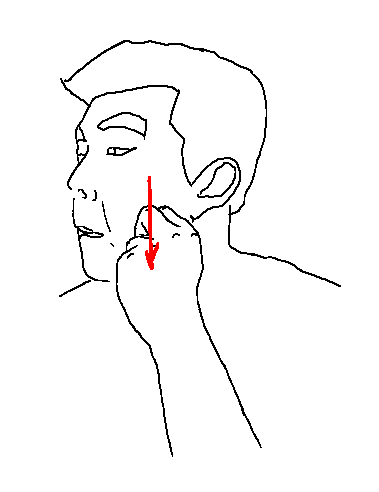
\includegraphics[width=\linewidth]{fig/老.pdf}
    %\caption{fig1}
    \end{minipage}%
    % \label{fig:}%
    }%
    \caption{}
    \label{fig:老}
\end{figure}

\begin{figure}[H]
    \centering
    \subfigure[]{
    \begin{minipage}[t]{0.33\linewidth}
    \centering
    \includegraphics[width=\linewidth]{fig/帅.pdf}
    %\caption{fig1}
    \end{minipage}%
    % \label{fig:}%
    }%
    \caption{}
    \label{fig:帅}
\end{figure}

\begin{figure}[H]
    \centering
    \subfigure[]{
    \begin{minipage}[t]{0.33\linewidth}
    \centering
    \includegraphics[width=\linewidth]{fig/外.pdf}
    %\caption{fig1}
    \end{minipage}%
    % \label{fig:}%
    }%
    \subfigure[]{
        \begin{minipage}[t]{0.33\linewidth}
        \centering
        \includegraphics[width=\linewidth]{fig/公.pdf}
        %\caption{fig1}
        \end{minipage}%
        % \label{fig:}%
    }%
    \caption{}
    \label{fig:外公}
\end{figure}

\begin{figure}[H]
    \centering
    \subfigure[]{
    \begin{minipage}[t]{0.33\linewidth}
    \centering
    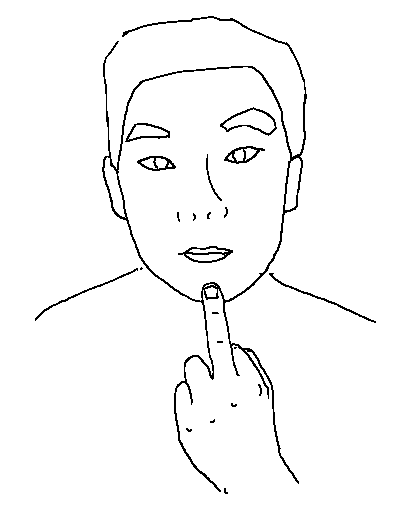
\includegraphics[width=\linewidth]{fig/中指.pdf}
    %\caption{fig1}
    \end{minipage}%
    % \label{fig:}%
    }%
    \subfigure[]{
        \begin{minipage}[t]{0.33\linewidth}
        \centering
        \includegraphics[width=\linewidth]{fig/男.pdf}
        %\caption{fig1}
        \end{minipage}%
        % \label{fig:}%
    }%
    \caption{}
    \label{fig:哥哥}
\end{figure}

\begin{figure}[H]
    \centering
    \subfigure[]{
    \begin{minipage}[t]{0.33\linewidth}
    \centering
    \includegraphics[width=\linewidth]{fig/父.pdf}
    %\caption{fig1}
    \end{minipage}%
    % \label{fig:}%
    }%
    \caption{}
    \label{fig:父}
\end{figure}

\begin{figure}[H]
    \centering
    \subfigure[]{
    \begin{minipage}[t]{0.33\linewidth}
    \centering
    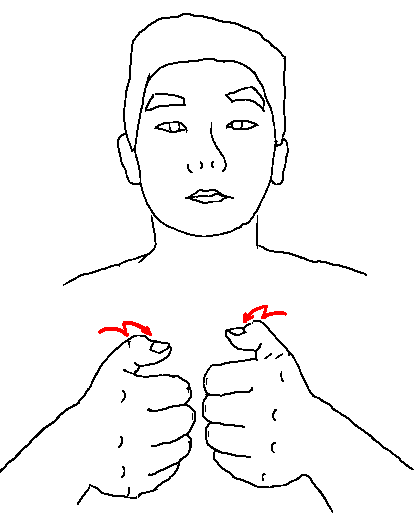
\includegraphics[width=\linewidth]{fig/爱人.pdf}
    %\caption{fig1}
    \end{minipage}%
    % \label{fig:}%
    }%
    \caption{}
    \label{fig:爱人}
\end{figure}

\begin{figure}[H]
    \centering
    \subfigure[]{
    \begin{minipage}[t]{0.33\linewidth}
    \centering
    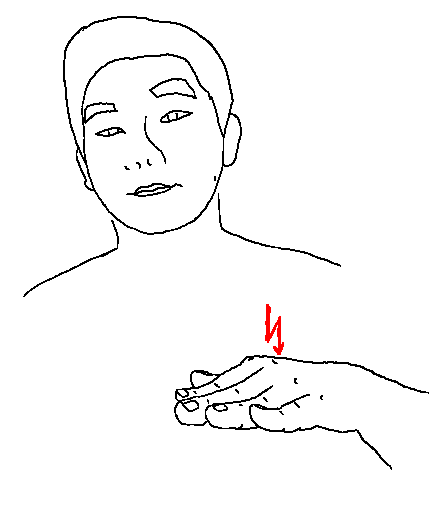
\includegraphics[width=\linewidth]{fig/小孩.pdf}
    %\caption{fig1}
    \end{minipage}%
    % \label{fig:}%
    }%
    \caption{}
    \label{fig:小孩}
\end{figure}

\begin{figure}[H]
    \centering
    \subfigure[]{
    \begin{minipage}[t]{0.33\linewidth}
    \centering
    \includegraphics[width=\linewidth]{fig/记.pdf}
    %\caption{fig1}
    \end{minipage}%
    % \label{fig:}%
    }%
    \caption{}
    \label{fig:记}
\end{figure}

\begin{figure}[H]
    \centering
    \subfigure[]{
    \begin{minipage}[t]{0.33\linewidth}
    \centering
    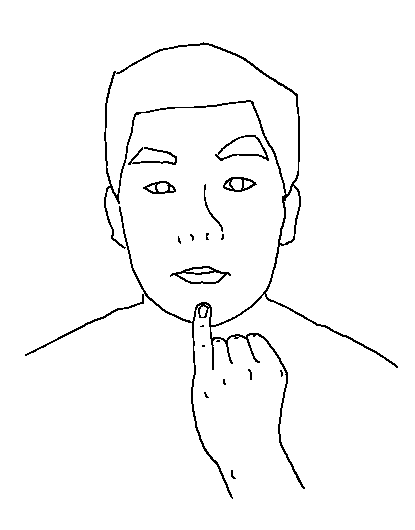
\includegraphics[width=\linewidth]{fig/小指.pdf}
    %\caption{fig1}
    \end{minipage}%
    % \label{fig:}%
    }%
    \subfigure[]{
        \begin{minipage}[t]{0.33\linewidth}
        \centering
        \includegraphics[width=\linewidth]{fig/女.pdf}
        %\caption{fig1}
        \end{minipage}%
        % \label{fig:}%
    }%
    \caption{}
    \label{fig:妹妹}
\end{figure}



\subsection{(b)问配图}

\begin{figure}[H]
    \centering
    \centering
    \subfigure[]{
    \begin{minipage}[t]{0.33\linewidth}
    \centering
    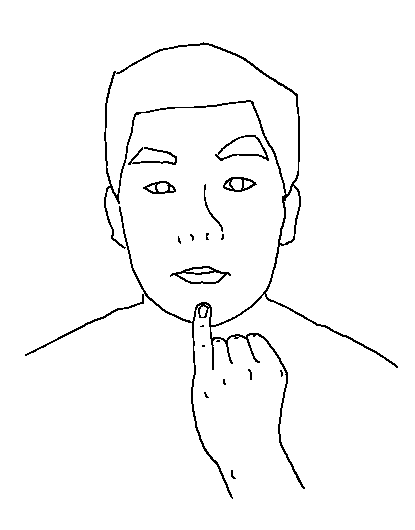
\includegraphics[width=\linewidth]{fig/小指.pdf}
    %\caption{fig1}
    \end{minipage}%
    % \label{fig:}%
    }%
    \subfigure[]{
        \begin{minipage}[t]{0.33\linewidth}
        \centering
        \includegraphics[width=\linewidth]{fig/男.pdf}
        %\caption{fig1}
        \end{minipage}%
        % \label{fig:}%
    }%
    \caption{}
    \label{fig:弟弟}
\end{figure}


\begin{figure}[H]
    \centering
    \subfigure[]{
        \begin{minipage}[t]{0.33\linewidth}
        \centering
        \includegraphics[width=\linewidth]{fig/表.pdf}
        %\caption{fig1}
        \end{minipage}%
        % \label{fig:}%
        }%
    \subfigure[]{
    \begin{minipage}[t]{0.33\linewidth}
    \centering
    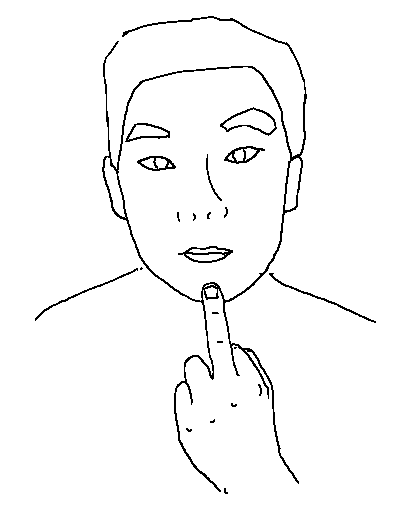
\includegraphics[width=\linewidth]{fig/中指.pdf}
    %\caption{fig1}
    \end{minipage}%
    % \label{fig:}%
    }%
    \subfigure[]{
        \begin{minipage}[t]{0.33\linewidth}
        \centering
        \includegraphics[width=\linewidth]{fig/女.pdf}
        %\caption{fig1}
        \end{minipage}%
        % \label{fig:}%
    }%
    \caption{}
    \label{fig:表姐}
\end{figure}

\begin{figure}[H]
    \centering
    \subfigure[]{
        \begin{minipage}[t]{0.33\linewidth}
        \centering
        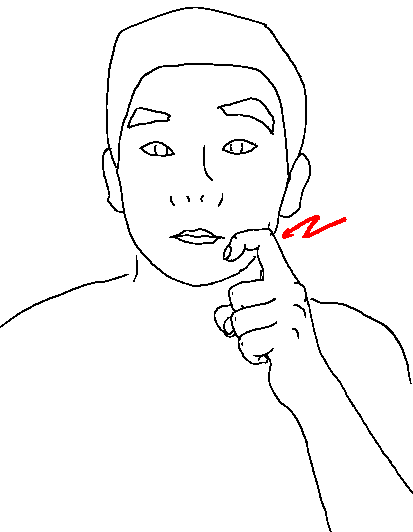
\includegraphics[width=\linewidth]{fig/舅舅.pdf}
        %\caption{fig1}
        \end{minipage}%
        % \label{fig:}%
        }%
    \caption{}
    \label{fig:舅舅}
\end{figure}

\begin{figure}[H]
    \centering
    \subfigure[]{
        \begin{minipage}[t]{0.33\linewidth}
        \centering
        \includegraphics[width=\linewidth]{fig/女.pdf}
        %\caption{fig1}
        \end{minipage}%
        % \label{fig:}%
        }%
    \subfigure[]{
    \begin{minipage}[t]{0.33\linewidth}
    \centering
    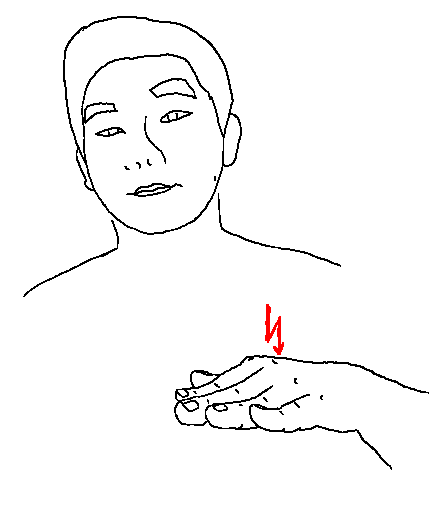
\includegraphics[width=\linewidth]{fig/小孩.pdf}
    %\caption{fig1}
    \end{minipage}%
    % \label{fig:}%
    }%
    \subfigure[]{
        \begin{minipage}[t]{0.33\linewidth}
        \centering
        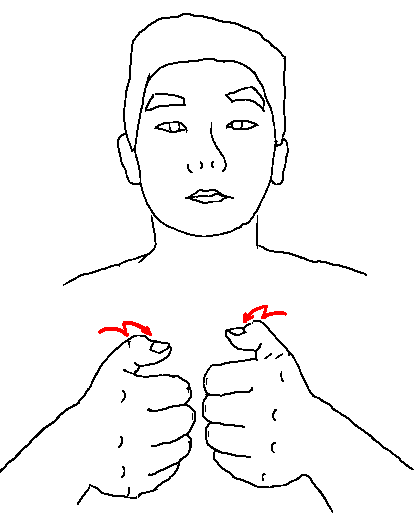
\includegraphics[width=\linewidth]{fig/爱人.pdf}
        %\caption{fig1}
        \end{minipage}%
        % \label{fig:}%
    }%
    \caption{}
    \label{fig:女婿}
\end{figure}

\begin{figure}[H]
    \centering
    \subfigure[]{
    \begin{minipage}[t]{0.33\linewidth}
    \centering
    \includegraphics[width=\linewidth]{fig/外.pdf}
    %\caption{fig1}
    \end{minipage}%
    % \label{fig:}%
    }%
    \subfigure[]{
    \begin{minipage}[t]{0.33\linewidth}
    \centering
    \includegraphics[width=\linewidth]{fig/生.pdf}
    %\caption{fig2}
    \end{minipage}%
    % \label{fig:}%
    }%
    \subfigure[]{
        \begin{minipage}[t]{0.33\linewidth}
        \centering
        \includegraphics[width=\linewidth]{fig/女.pdf}
        %\caption{fig2}
        \end{minipage}%
    % \label{fig:}%
    }%
    \caption{}
    \label{fig:外甥女}
\end{figure}

\begin{figure}[H]
    \centering
    \subfigure[]{
        \begin{minipage}[t]{0.33\linewidth}
        \centering
        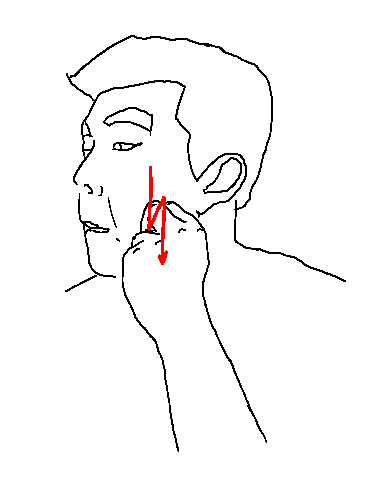
\includegraphics[width=\linewidth]{fig/姥姥.pdf}
        %\caption{fig1}
        \end{minipage}%
        % \label{fig:}%
        }%
    \caption{}
    \label{fig:姥姥}
\end{figure}

\begin{figure}[H]
    \centering
    \subfigure[]{
        \begin{minipage}[t]{0.33\linewidth}
        \centering
        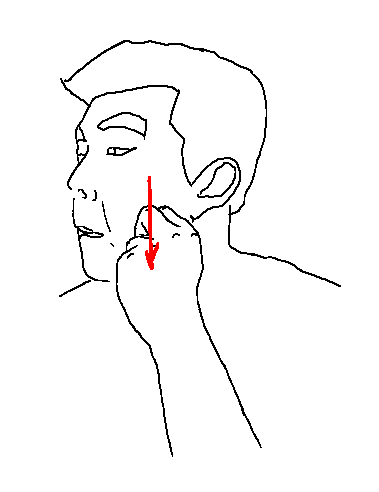
\includegraphics[width=\linewidth]{fig/老.pdf}
        %\caption{fig1}
        \end{minipage}%
        % \label{fig:}%
        }%
    \subfigure[]{
        \begin{minipage}[t]{0.33\linewidth}
        \centering
        \includegraphics[width=\linewidth]{fig/爷.pdf}
        %\caption{fig1}
        \end{minipage}%
        % \label{fig:}%
        }%
    \caption{}
    \label{fig:姥爷}
\end{figure}

\begin{figure}[H]
    \centering
    \subfigure[]{
        \begin{minipage}[t]{0.33\linewidth}
        \centering
        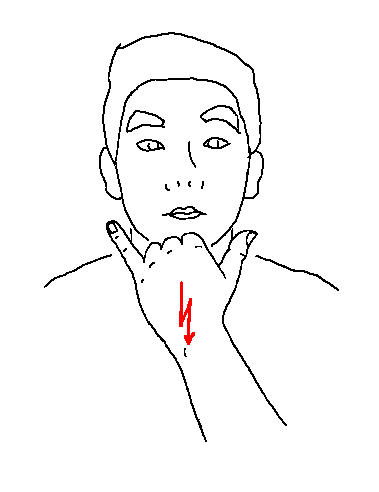
\includegraphics[width=\linewidth]{fig/爷爷.pdf}
        %\caption{fig1}
        \end{minipage}%
        % \label{fig:}%
        }%
    \caption{}
    \label{fig:爷爷}
\end{figure}

\begin{figure}[H]
    \centering
    \subfigure[]{
        \begin{minipage}[t]{0.33\linewidth}
        \centering
        \includegraphics[width=\linewidth]{fig/姨.pdf}
        %\caption{fig1}
        \end{minipage}%
        % \label{fig:}%
        }%
    \subfigure[]{
        \begin{minipage}[t]{0.33\linewidth}
        \centering
        \includegraphics[width=\linewidth]{fig/父.pdf}
        %\caption{fig1}
        \end{minipage}%
        % \label{fig:}%
        }%
    \caption{}
    \label{fig:姨父}
\end{figure}

\begin{figure}[H]
    \centering
    \subfigure[]{
        \begin{minipage}[t]{0.33\linewidth}
        \centering
        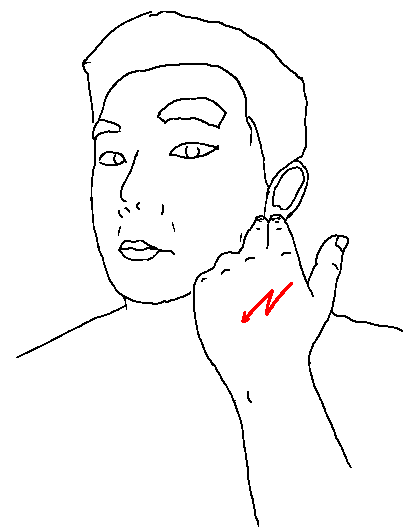
\includegraphics[width=\linewidth]{fig/婶婶.pdf}
        %\caption{fig1}
        \end{minipage}%
        % \label{fig:}%
        }%
    \caption{}
    \label{fig:婶婶}
\end{figure}

\begin{figure}[H]
    \centering
    \subfigure[]{
        \begin{minipage}[t]{0.33\linewidth}
        \centering
        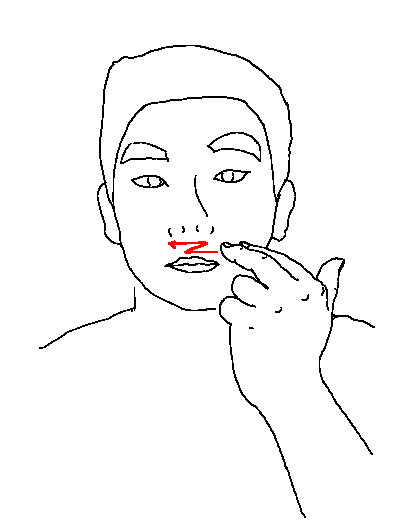
\includegraphics[width=\linewidth]{fig/叔叔.pdf}
        %\caption{fig1}
        \end{minipage}%
        % \label{fig:}%
        }%
    \caption{}
    \label{fig:叔叔}
\end{figure}

\begin{figure}[H]
    \centering
    \subfigure[]{
        \begin{minipage}[t]{0.33\linewidth}
        \centering
        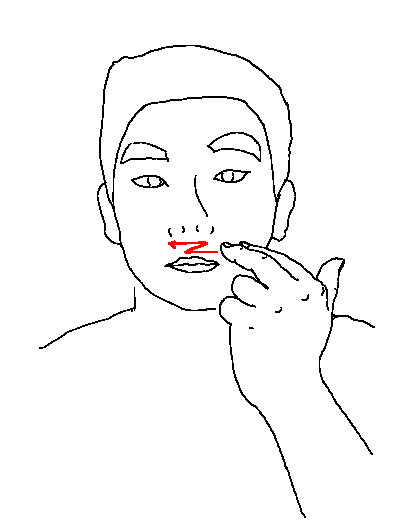
\includegraphics[width=\linewidth]{fig/叔叔.pdf}
        %\caption{fig1}
        \end{minipage}%
        % \label{fig:}%
        }%
    \subfigure[]{
        \begin{minipage}[t]{0.33\linewidth}
        \centering
        \includegraphics[width=\linewidth]{fig/父.pdf}
        %\caption{fig1}
        \end{minipage}%
        % \label{fig:}%
        }%
    \caption{}
    \label{fig:叔父}
\end{figure}


% \subsection{答案}


% 妹妹(小指+女)
% 哥哥(中指+男)
% 男
% 记忆(J)
% 父亲
% 丈夫/妻子/爱人
% 小孩->
% 外公-》
% 老->
% 帅

% 手语词汇填空:
% 弟弟(小指+男)、表姐(表+中指+女)
% 舅舅(J+J)
% 女婿(女+小孩+爱人)
% 外甥女(外+分娩+女)
% 姥爷(老+Y)、爷爷(Y+Y)、姨父(Y+父)
% 婶婶、叔叔(手指拼音)


\end{document}

